\section{Discussion and Interpretation}
% [WRITING GUIDANCE]
% Target length: 1 column.
% Interpret the results in a business context.
% Do NOT fabricate interpretations; base them on the SHAP or Feature Importance plots.

% Insert Figure 6 here. (Feature Importance)
\begin{figure}[htbp]
\centerline{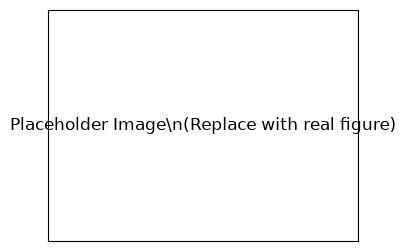
\includegraphics[width=\columnwidth]{figures/placeholder.png}}
\caption{Feature Importance Ranking of the best ensemble model.}
\label{fig:feat_imp}
\end{figure}

% Insert Figure 7 here. (SHAP Summary)
\begin{figure}[htbp]
\centerline{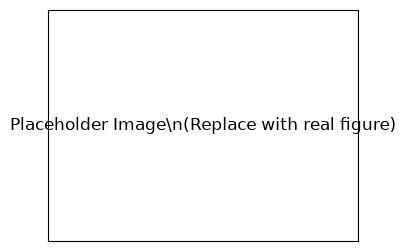
\includegraphics[width=\columnwidth]{figures/placeholder.png}}
\caption{SHAP Summary Plot illustrating directional impact of features.}
\label{fig:shap}
\end{figure}

% Insert Feature Importance Ranking Table
\begin{table}[htbp]
\caption{Top 5 Most Important Features}
\begin{center}
\begin{tabular}{|c|l|}
\hline
\textbf{Rank} & \textbf{Feature Name} \\
\hline
1 & Customer\_Value\_Score \\
2 & Campaign\_Acceptance\_Count \\
3 & Recency \\
4 & ... \\
5 & ... \\
\hline
\end{tabular}
\label{tab:feat_ranking}
\end{center}
\end{table}

% Discuss what these features mean for the marketing department.
% Write your discussion here...
